\documentclass{article}

\usepackage{tikz}
\usetikzlibrary{automata, positioning}
\begin{document}
\begin{tikzpicture}[shorten >= 1pt, node distance = 2.5cm, on grid, auto]
  \node[state, initial] (0) {0};
  \node[state] (1) [right=of 0] {1};
  \node[state] (2) [above right=of 1] {2};
  \node[state] (3) [below right=of 1] {3};
  \node[state] (4) [right=of 2] {4};
  \node[state] (5) [right=of 3] {5};
  \node[state] (6) [below right=of 4] {6};
  \node[state] (7) [right=of 6] {7};
  \node[state] (8) [right=of 7] {8};
  \node[state] (9) [below=6cm of 8] {9};
  \node[state] (10) [left=of 9] {10};
  \node[state] (11) [left=of 10] {11};
  \node[state] (12) [above left=of 11] {12};
  \node[state] (13) [below left=of 11] {13};
  \node[state] (14) [left=of 12] {14};
  \node[state] (15) [left=of 13] {15};
  \node[state] (16) [below left=of 14] {16};
  \node[state, accepting] (17) [left=of 16] {17};
  \path[->]
    (0) edge node {$\epsilon$} (1)
        edge [bend right=50] node {$\epsilon$} (7)
    (1) edge node {$\epsilon$} (2)
        edge node {$\epsilon$} (3)
    (2) edge node {a} (4)
    (3) edge node {b} (5)
    (4) edge node {$\epsilon$} (6)
    (5) edge node {$\epsilon$} (6)
    (6) edge node {$\epsilon$} (7)
        edge [bend right=80, looseness=1.5] node {$\epsilon$} (1)
    (7) edge node {a} (8)
    (8) edge node {b} (9)
    (9) edge node {b} (10)
    (10) edge node {$\epsilon$} (11)
        edge [bend left=50] node {$\epsilon$} (17)
    (11) edge node {$\epsilon$} (12)
        edge node {$\epsilon$} (13)
    (12) edge node {a} (14)
    (13) edge node {b} (15)
    (14) edge node {$\epsilon$} (16)
    (15) edge node {$\epsilon$} (16)
    (16) edge node {$\epsilon$} (17)
        edge [bend left=80, looseness=1.5] node {$\epsilon$} (11);
\end{tikzpicture}

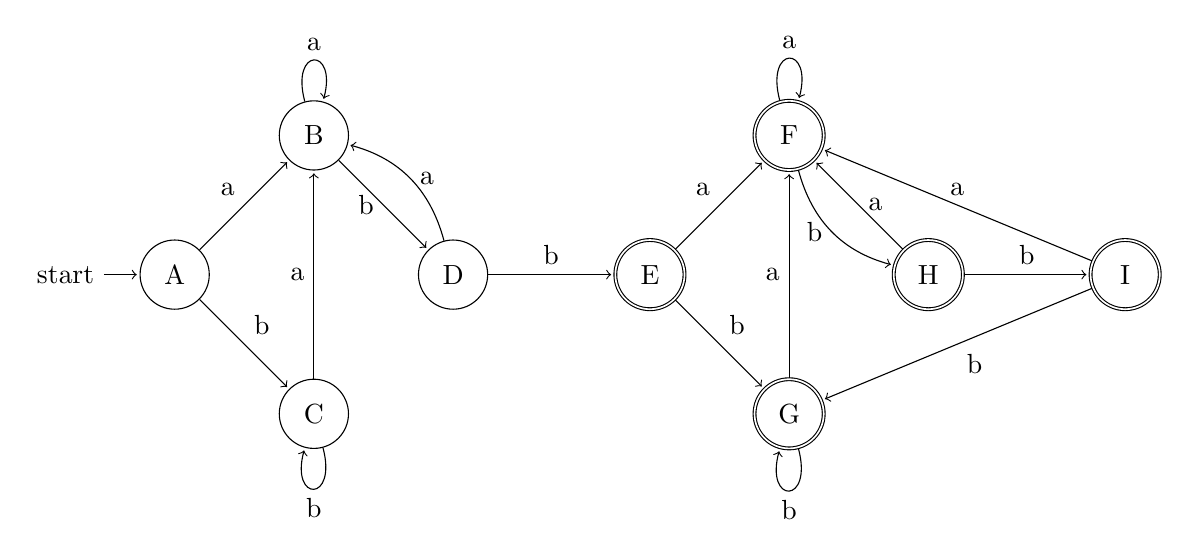
\begin{tikzpicture}[shorten >= 1pt, node distance = 2.5cm, on grid, auto]
  \node[state, initial] (A) {A};
  \node[state] (B) [above right=of A] {B};
  \node[state] (C) [below right=of A] {C};
  \node[state] (D) [below right=of B] {D};
  \node[state, accepting] (E) [right=of D] {E};
  \node[state, accepting] (F) [above right=of E] {F};
  \node[state, accepting] (G) [below right=of E] {G};
  \node[state, accepting] (H) [below right=of F] {H};
  \node[state, accepting] (I) [right=of H] {I};
  \path[->]
    (A) edge node {a} (B)
        edge node {b} (C)
    (B) edge [loop above] node {a} (B)
        edge node [left] {b} (D)
    (C) edge node {a} (B)
        edge [loop below] node {b} (C)
    (D) edge [bend right] node [right] {a} (B)
        edge node {b} (E)
    (E) edge node {a} (F)
        edge node {b} (G)
    (F) edge [loop above] node {a} (F)
        edge [bend right] node [left] {b} (H)
    (G) edge node {a} (F)
        edge [loop below] node {b} (G)
    (H) edge node [right] {a} (F)
        edge node {b} (I)
    (I) edge node [above] {a} (F)
        edge node {b} (G);
\end{tikzpicture}
\end{document}
